
\documentclass[11pt]{beamer}

% Theme choice:
\usetheme{NIU}

% Packages
\usepackage{epstopdf}
\usepackage{graphicx}
\usepackage{graphics}
\usepackage[style=authoryear-ibid, natbib, maxcitenames=3,
giveninits, backend=biber, urldate=long]{biblatex}
\addbibresource{beamer.bib}

% Title page details: 
\title{Analysis of the 2020 US election results}
\author{Shaibu Yahaya}
\institute{Northern Illinois University}
\date{\today}

% Title Graphics
\titlegraphic{
\includegraphics[height=2.5cm]{NIU_logo.eps}}

\begin{document}

%%%%%%%%%%%%%%%%%%%%%%%%%%%%%%%%%%% Title page
\maketitle


%%%%%%%%%%%%%%%%%%%%%%%%%%%%%%%%%%% Slide 1: Table of Contents
\begin{frame}{Table of Contents}
\begin{itemize}
    \item Introduction
    \item Descriptions of States
    \item Change in Republican results (2016 vs 2020)
    \item Change in Democrats results (2016 vs 2020)
    \item Regression results for change in Republican votes
    \item Regression results for change in Democrats votes
    \item What the regression results mean for elections going forward
    \item References
\end{itemize}
\end{frame}


%%%%%%%%%%%%%%%%%%%%%%%%%%%%%%%%%%% Slide 2: Intro
\begin{frame}{Introduction}
\begin{itemize}
\item In this presentation, we want to analyze the results of the US 2020 election in 5 US MidWest states.
\item We compare this to the 2016 elections and the demography of these states.
\item Only the Republican and Democratic presidential results are considered.
\item The 2020 election data was obtained from the Harvard Dataverse, the 2016 election data was scraped using the New York Times API, and the census data was obtained from the tidycensus API in R software.
\item The figures and tables were generated using the R software.
\end{itemize}
\end{frame}

%%%%%%%%%%%%%%%%%%%%%%%%%%%%%%%%%%% Slide 3-7: Describe states
\begin{frame}[shrink=0.4]{Description of States}
\textbf{Iowa}
    \begin{figure}
\centering
\caption{\label{iowa}}
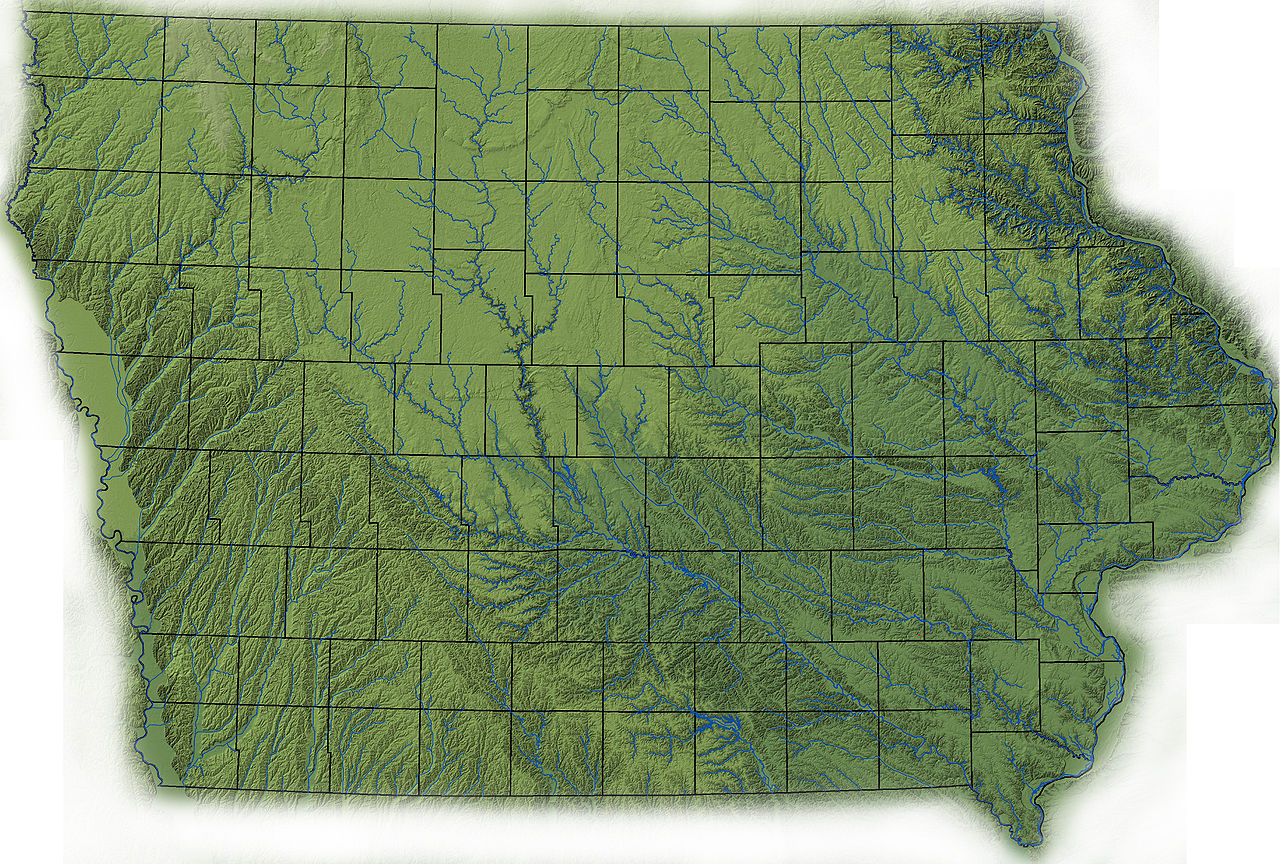
\includegraphics[%
    width=0.2\textwidth]{iowa.jpeg}
\end{figure}
\begin{itemize}
    \item Population of about 3.2 million. 
    \item The capital is  Des Moines and the major cities are Des Moines, Cedar Rapids, and Davenport. 
    \item Its largest industries are agriculture, insurance and financial services, biotechnology, and manufacturing.
\end{itemize}
\end{frame}

\begin{frame}[shrink=0.4]{Description of States}
\textbf{Minnesota}
    \begin{figure}
\centering
\caption{\label{Minnesota}}
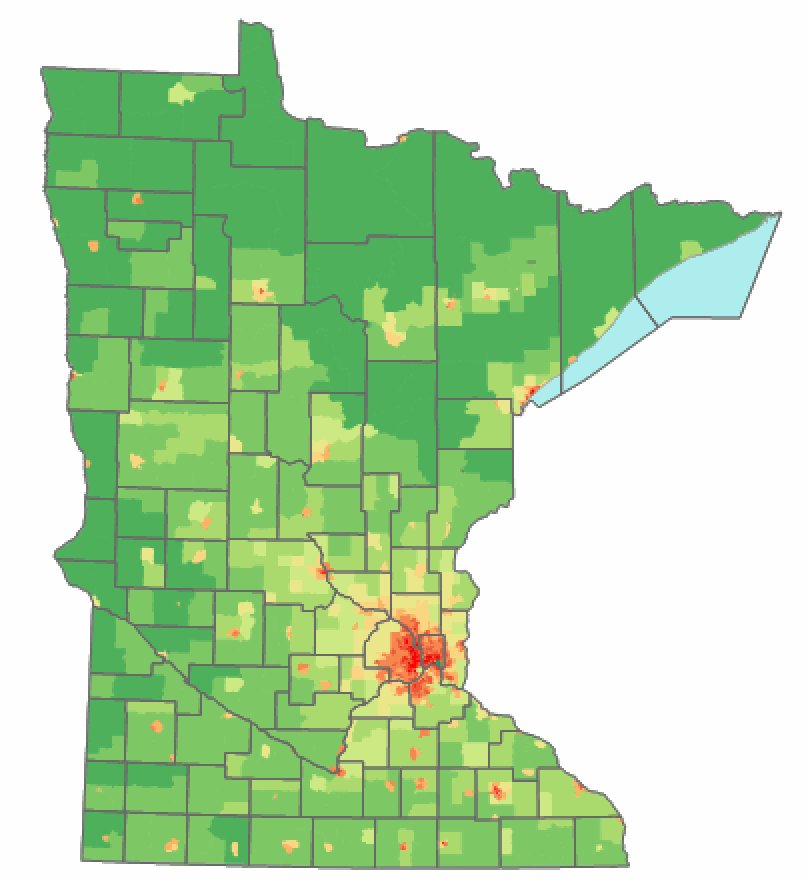
\includegraphics[%
    width=0.2\textwidth]{minnesota.png}
\end{figure}
\begin{itemize}
    \item Population of about 5.7 million. 
    \item The capital is  Saint Paul and the major cities are Minneapolis, Saint Paul, Rochester and Duluth. 
    \item Its largest industries are agriculture, manufacturing, mining and energy production.
\end{itemize}
\end{frame}

\begin{frame}[shrink=0.4]{Description of States}
\textbf{North Dakota}
    \begin{figure}
\centering
\caption{\label{nd}}
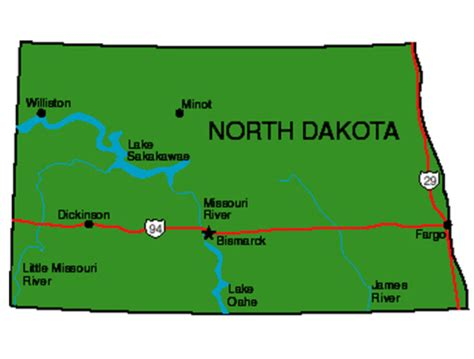
\includegraphics[%
    width=0.2\textwidth]{nd.jpeg}
\end{figure}
\begin{itemize}
    \item Population of about 779,000. 
    \item The capital is Bismarck and the largest cities include Fargo, Bismarck, Grand Forks and Minot.
    \item Its key industries are agriculture, energy and natural resources,and autonomous systems.
\end{itemize}
\end{frame}

\begin{frame}[shrink=0.4]{Description of States}
\textbf{South Dakota}
    \begin{figure}
\centering
\caption{\label{sd}}
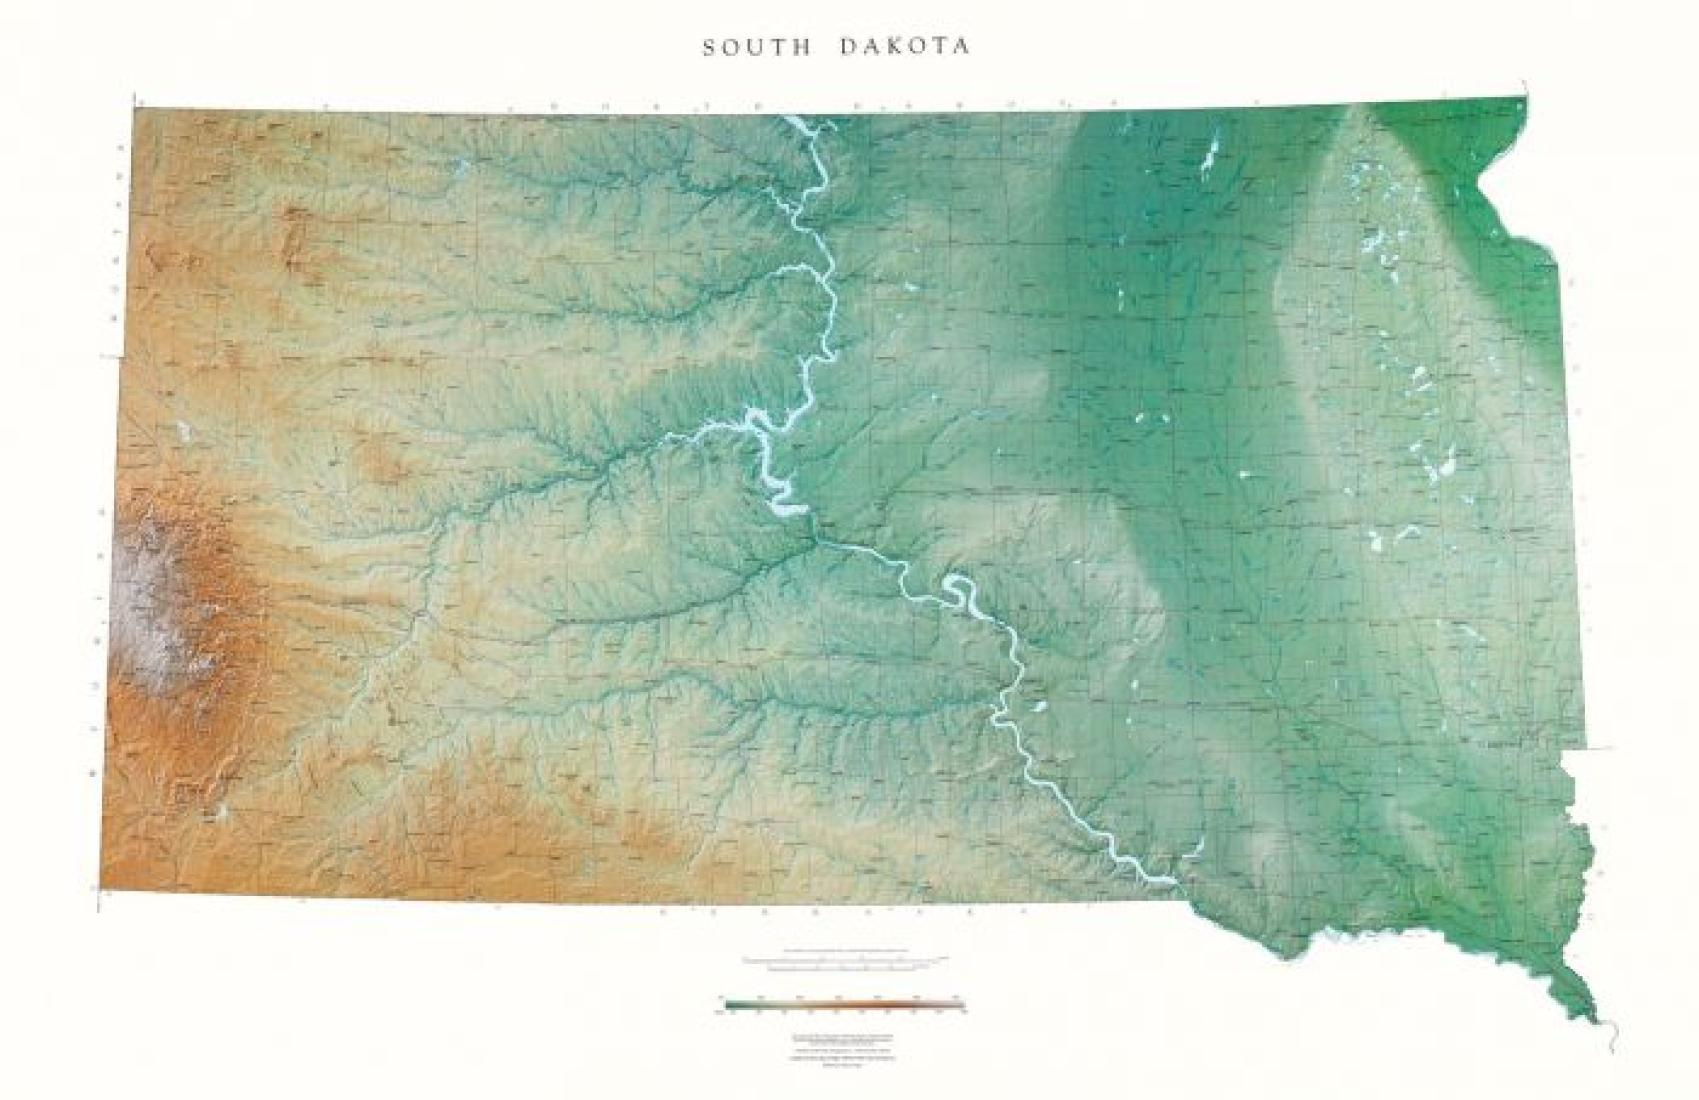
\includegraphics[%
    width=0.2\textwidth]{sd.jpeg}
\end{figure}
\begin{itemize}
    \item Population of about 887,000. 
    \item The capital is  Pierre and the major cities are Sioux Falls, Rapid City, Aberdeen and Brookings. 
    \item Its largest industries are agriculture, manufacturing and mining.
\end{itemize}
\end{frame}

\begin{frame}[shrink=0.4]{Description of States}
\textbf{Wisconsin}
    \begin{figure}
\centering
\caption{\label{wisconsin}}
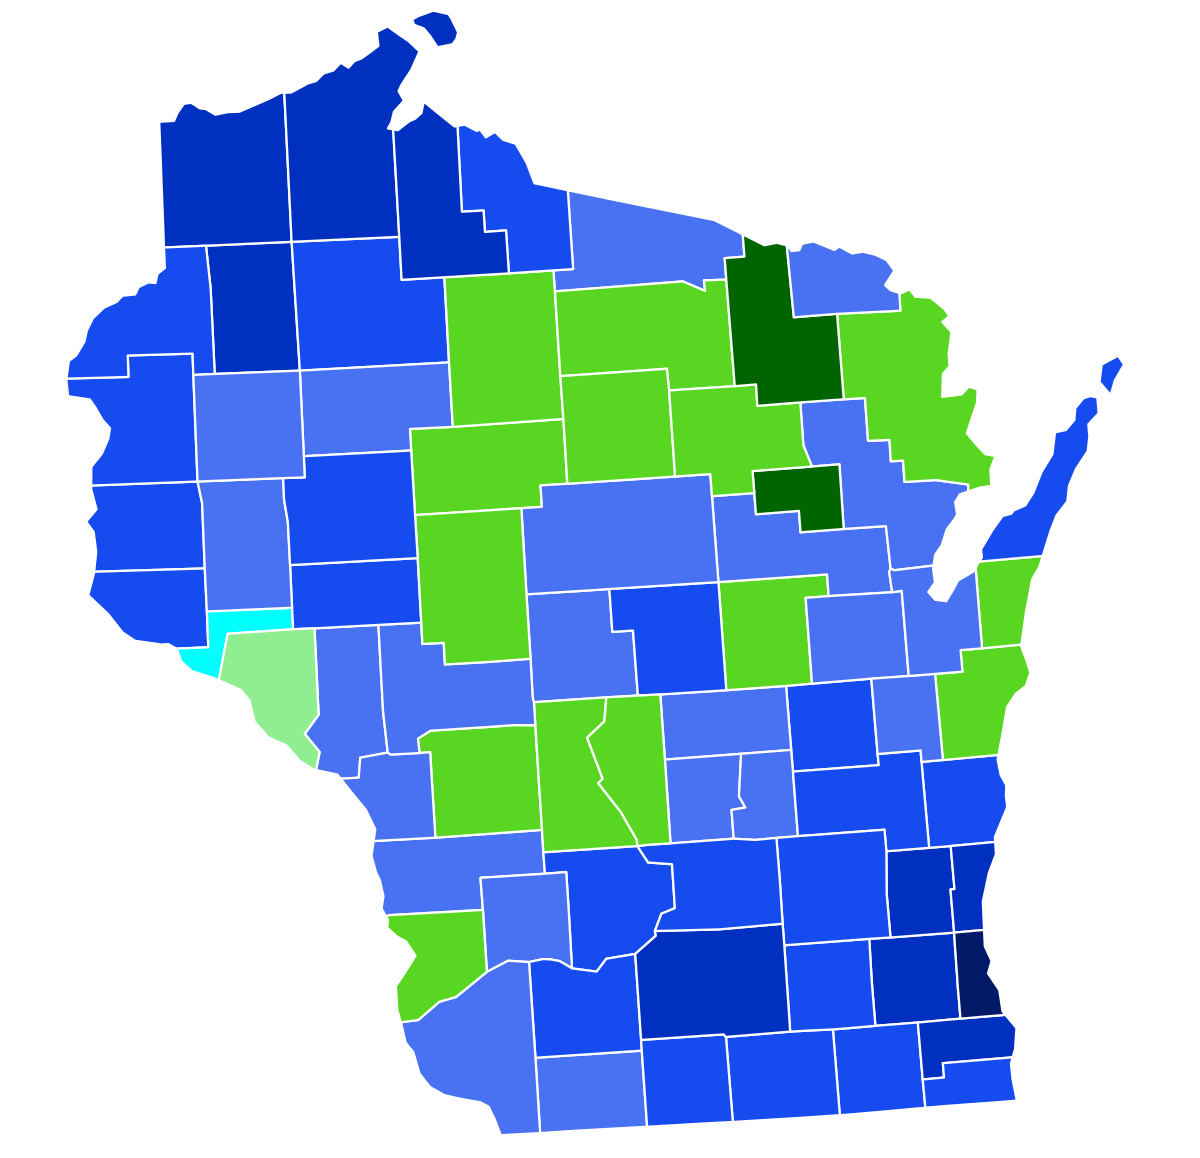
\includegraphics[%
    width=0.2\textwidth]{wisconsin.png}
\end{figure}
\begin{itemize}
    \item Population of about 5.9 million. 
    \item The capital is  Madison and the major cities are Milwaukee, Madison, Green Bay and Kenosha. 
    \item Its largest industries are manufacturing, agriculture, health care and tourism.
\end{itemize}
\end{frame}

%%%%%%%%%%%%%%%%%%%%%%%%%%%%%%%%%%% Slide 8: Rep votes changes
\begin{frame}{Change in Republican results (2016 vs 2020)}
\begin{figure}%[h]
\centering
\caption{\label{rep}}
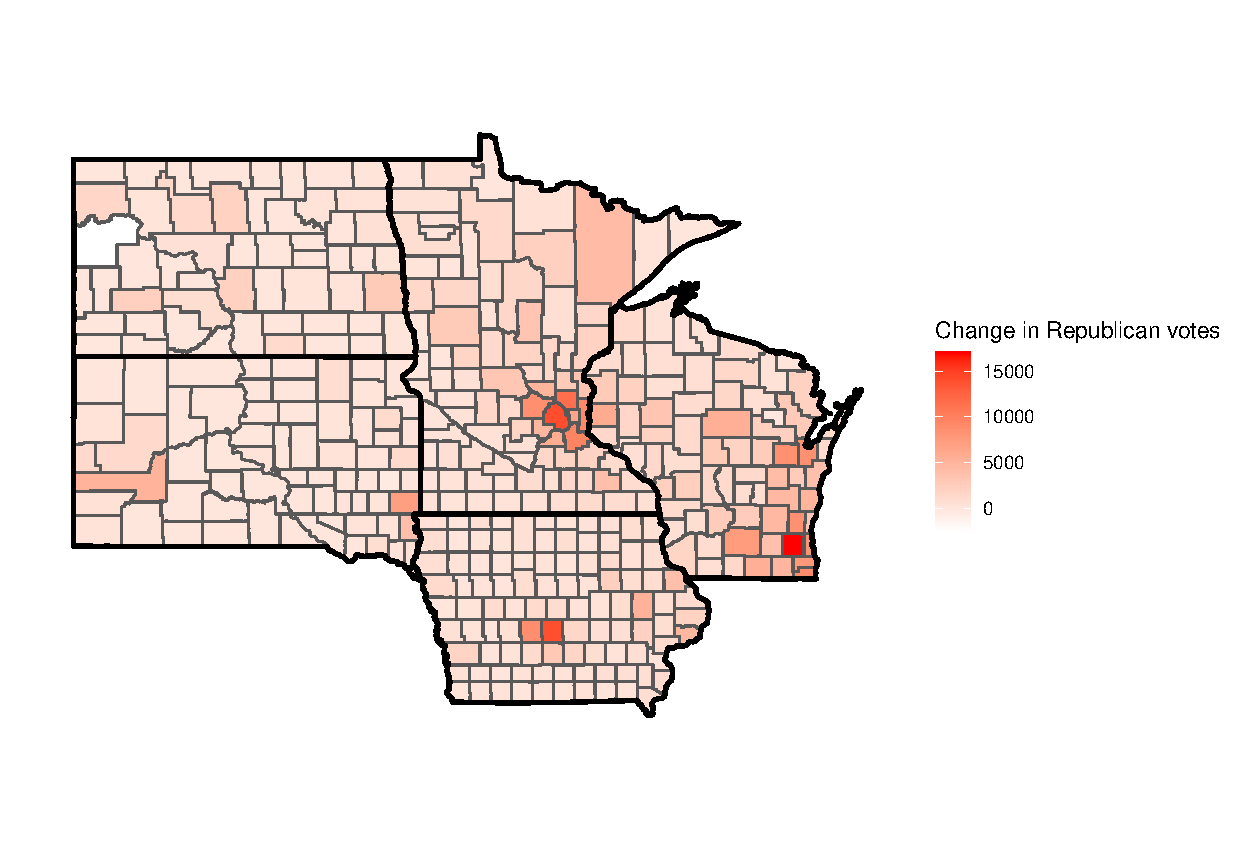
\includegraphics[%
    width=0.4\textwidth]{rep.eps}
\end{figure}
There was more than 20 million votes in 2020 compared to 2016 and this reflected in positive changes in votes in almost all counties considered. However, the maximum votes change in the counties considered was just 17,106 with the minimum being -2,517.

\end{frame}

%%%%%%%%%%%%%%%%%%%%%%%%%%%%%%%%%%% Slide 9: Dem votes changes
\begin{frame}{Change in Democrats results (2016 vs 2020)}
\begin{figure}
\centering
\caption{\label{dem}}
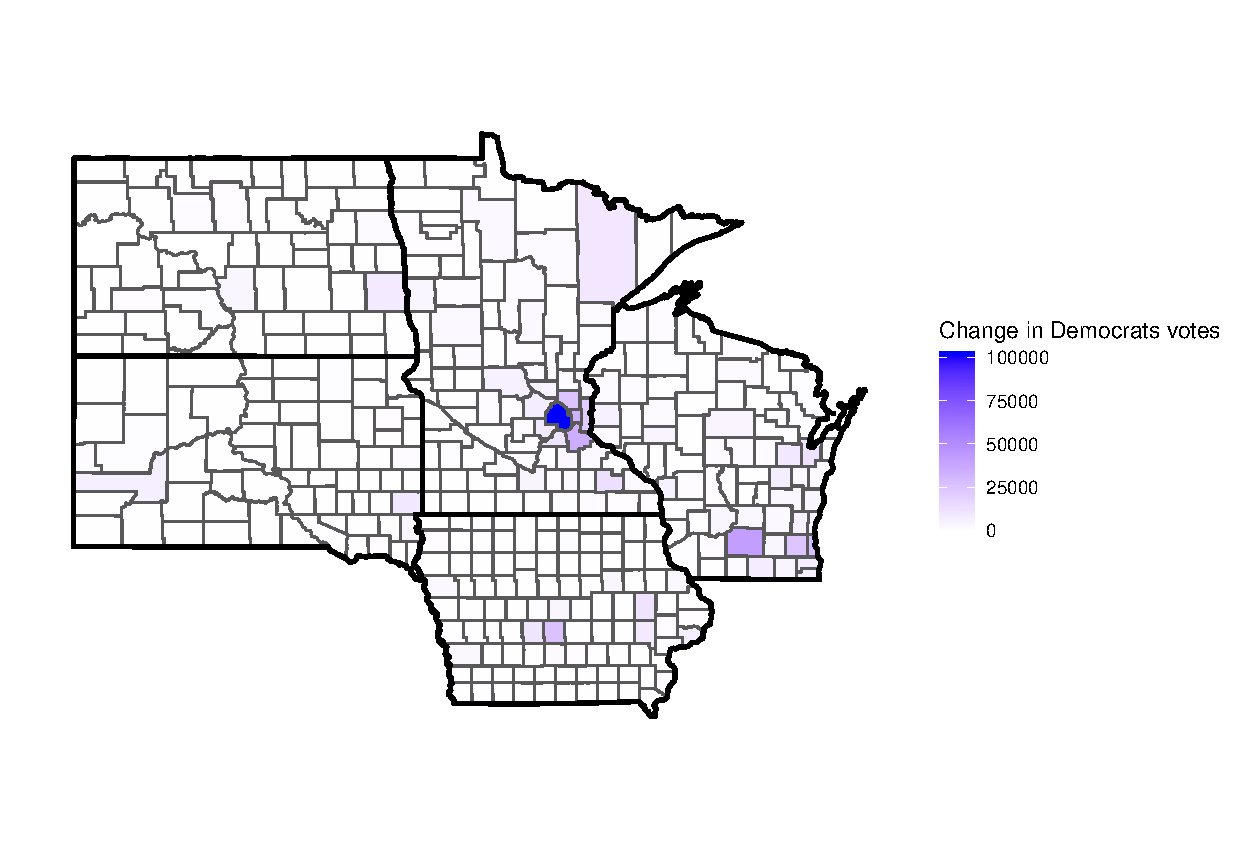
\includegraphics[%
    width=0.4\textwidth]{dem.eps}
\end{figure}
In the case of the Democrats, the maximum vote change was 103,335 and the minimum is -437. The Democrats won the election by gaining more votes and losing less votes.
\end{frame}

%%%%%%%%%%%%%%%%%%%%%%%%%%%%%%%%%%% Slide 10: Rep regression
\begin{frame}[shrink=62]{Regression results for change in Republican's votes}
\centering
\begin{table}
  \caption{} 
  \label{Regression 1} 
\begin{tabular}{@{\extracolsep{5pt}}lc} 
\\[-1.8ex]\hline 
\hline \\[-1.8ex] 
 & \multicolumn{1}{c}{\textit{Dependent variable:}} \\ 
\cline{2-2} 
\\[-1.8ex] & c\_Republicans \\ 
\hline \\[-1.8ex] 
 pc\_White & $-$102.517$^{*}$ \\ 
  & (56.460) \\ 
  & \\ 
 pc\_Male & $-$30.393 \\ 
  & (58.134) \\ 
  & \\ 
 factor(state)iowa & 955.582$^{***}$ \\ 
  & (211.892) \\ 
  & \\ 
 factor(state)minnesota & 1,738.199$^{***}$ \\ 
  & (234.685) \\ 
  & \\ 
 factor(state)north-dakota & 257.497 \\ 
  & (290.363) \\ 
  & \\ 
 factor(state)south-dakota & 454.750$^{*}$ \\ 
  & (259.066) \\ 
  & \\ 
 factor(state)wisconsin & 2,809.685$^{***}$ \\ 
  & (246.251) \\ 
  & \\ 
\hline \\[-1.8ex]
Observations & 377 \\ 
R$^{2}$ & 0.390 \\ 
Adjusted R$^{2}$ & 0.378 \\ 
Residual Std. Error & 2,080.084 (df = 370) \\ 
F Statistic & 33.788$^{***}$ (df = 7; 370) \\ 
\hline 
\hline \\[-1.8ex] 
\textit{Note:}  & \multicolumn{1}{r}{$^{*}$p$<$0.1; $^{**}$p$<$0.05; $^{***}$p$<$0.01} \\ 
\end{tabular} 
\end{table} 
\end{frame}

%%%%%%%%%%%%%%%%%%%%%%%%%%%%%%%%%%% Slide 11: Dem regression
\begin{frame}[shrink=62]{Regression results for change in Democrats' votes}
\begin{table}
  \caption{} 
  \label{Regression 2}
\begin{tabular}{@{\extracolsep{5pt}}lc} 
\\[-1.8ex]\hline 
\hline \\[-1.8ex] 
 & \multicolumn{1}{c}{\textit{Dependent variable:}} \\ 
\cline{2-2} 
\\[-1.8ex] & c\_Democrats \\ 
\hline \\[-1.8ex] 
 pc\_White & $-$316.264$^{*}$ \\ 
  & (188.400) \\ 
  & \\ 
 pc\_Male & $-$9.242 \\ 
  & (193.987) \\ 
  & \\ 
 factor(state)iowa & 868.818 \\ 
  & (707.058) \\ 
  & \\ 
 factor(state)minnesota & 3,642.763$^{***}$ \\ 
  & (783.116) \\ 
  & \\ 
 factor(state)north-dakota & 105.826 \\ 
  & (968.905) \\ 
  & \\ 
 factor(state)south-dakota & 319.648 \\ 
  & (864.470) \\ 
  & \\ 
 factor(state)wisconsin & 3,329.195$^{***}$ \\ 
  & (821.710) \\ 
  & \\ 
\hline \\[-1.8ex] 
Observations & 377 \\ 
R$^{2}$ & 0.124 \\ 
Adjusted R$^{2}$ & 0.108 \\ 
Residual Std. Error & 6,940.987 (df = 370) \\ 
F Statistic & 7.515$^{***}$ (df = 7; 370) \\ 
\hline 
\hline \\[-1.8ex] 
\textit{Note:}  & \multicolumn{1}{r}{$^{*}$p$<$0.1; $^{**}$p$<$0.05; $^{***}$p$<$0.01} \\ 
\end{tabular} 
\end{table} 
\end{frame}

%%%%%%%%%%%%%%%%%%%%%%%%%%%%%%%%%%% Slide 12-13: Implications
\begin{frame}{What the regression results mean for elections going forward}
\begin{itemize}

\item From the tables above, a percentage change in White population negatively and significantly affected the change in votes of both Republicans and Democrats. However, the Democrats were affected more. According to an article on Asam News, White population "feel like a minority group that is in decline, and they feel that people of color are rising while they are declining” (Sohrabji, 2020). Trump's policies were perceived as anti-immigration and the White population therefore identifies with him more.

\item A percentage change in Male population also negatively and but insignificantly affect the change in votes of both Republicans and Democrats. But the Democrats were less affected.

\end{itemize}
\end{frame}

\begin{frame}{What the regression results mean for elections going forward}
\begin{itemize}

\item Minnesota and Wisconsin have positive and significant effects on the vote change for Republicans and Democrats. A lot of attention should be given to these states.

\item Iowa has a positive and significant effect on Republican votes but positive and insignificant effect on Democrat votes.

\item Going forward, both parties need to develop strategies on how to allay the fears of the White population and make them feel the country belongs to them. The male population also deserve attention especially in terms of more job creation.

\end{itemize}
\end{frame}

%%%%%%%%%%%%%%%%%%%%%%%%%%%%%%%%%%% Slide 14: Refs
\begin{frame}{References}
\begin{thebibliography}{10}
\setbeamertemplate{bibliography item}[text]

\bibitem{nytimes}
The Associated Press (2018). 2016 Presidential Election Results. The New York Times. URL:https://www.nytimes.com/elections/2016/results/president. (Accessed on 2021-28-09)

\bibitem{mit}
Harvard Dataverse (2018). County Presidential Election Returns 2000-2020. MIT Election Data and Science Lab. URL:https://doi.org/10.7910/DVN/VOQCHQ. (Accessed on 2021-28-09)

\bibitem{asam}
Sohrabji, Sunita (2020). Why Whites voted for Trump: They feel like a minority. Asam News. URL:https://asamnews.com/2020/12/17/three-out-of-five-white-voters-voted-for-trump/. (Accessed on 2021-28-09)

\end{thebibliography}
\end{frame}

%%%%%%%%%%%%%%%%%%%%%%%%%%%%%%%%%%% Slide 15: Thanks
\begin{frame}{Thank You}
%\begin{wrapfigure}
%    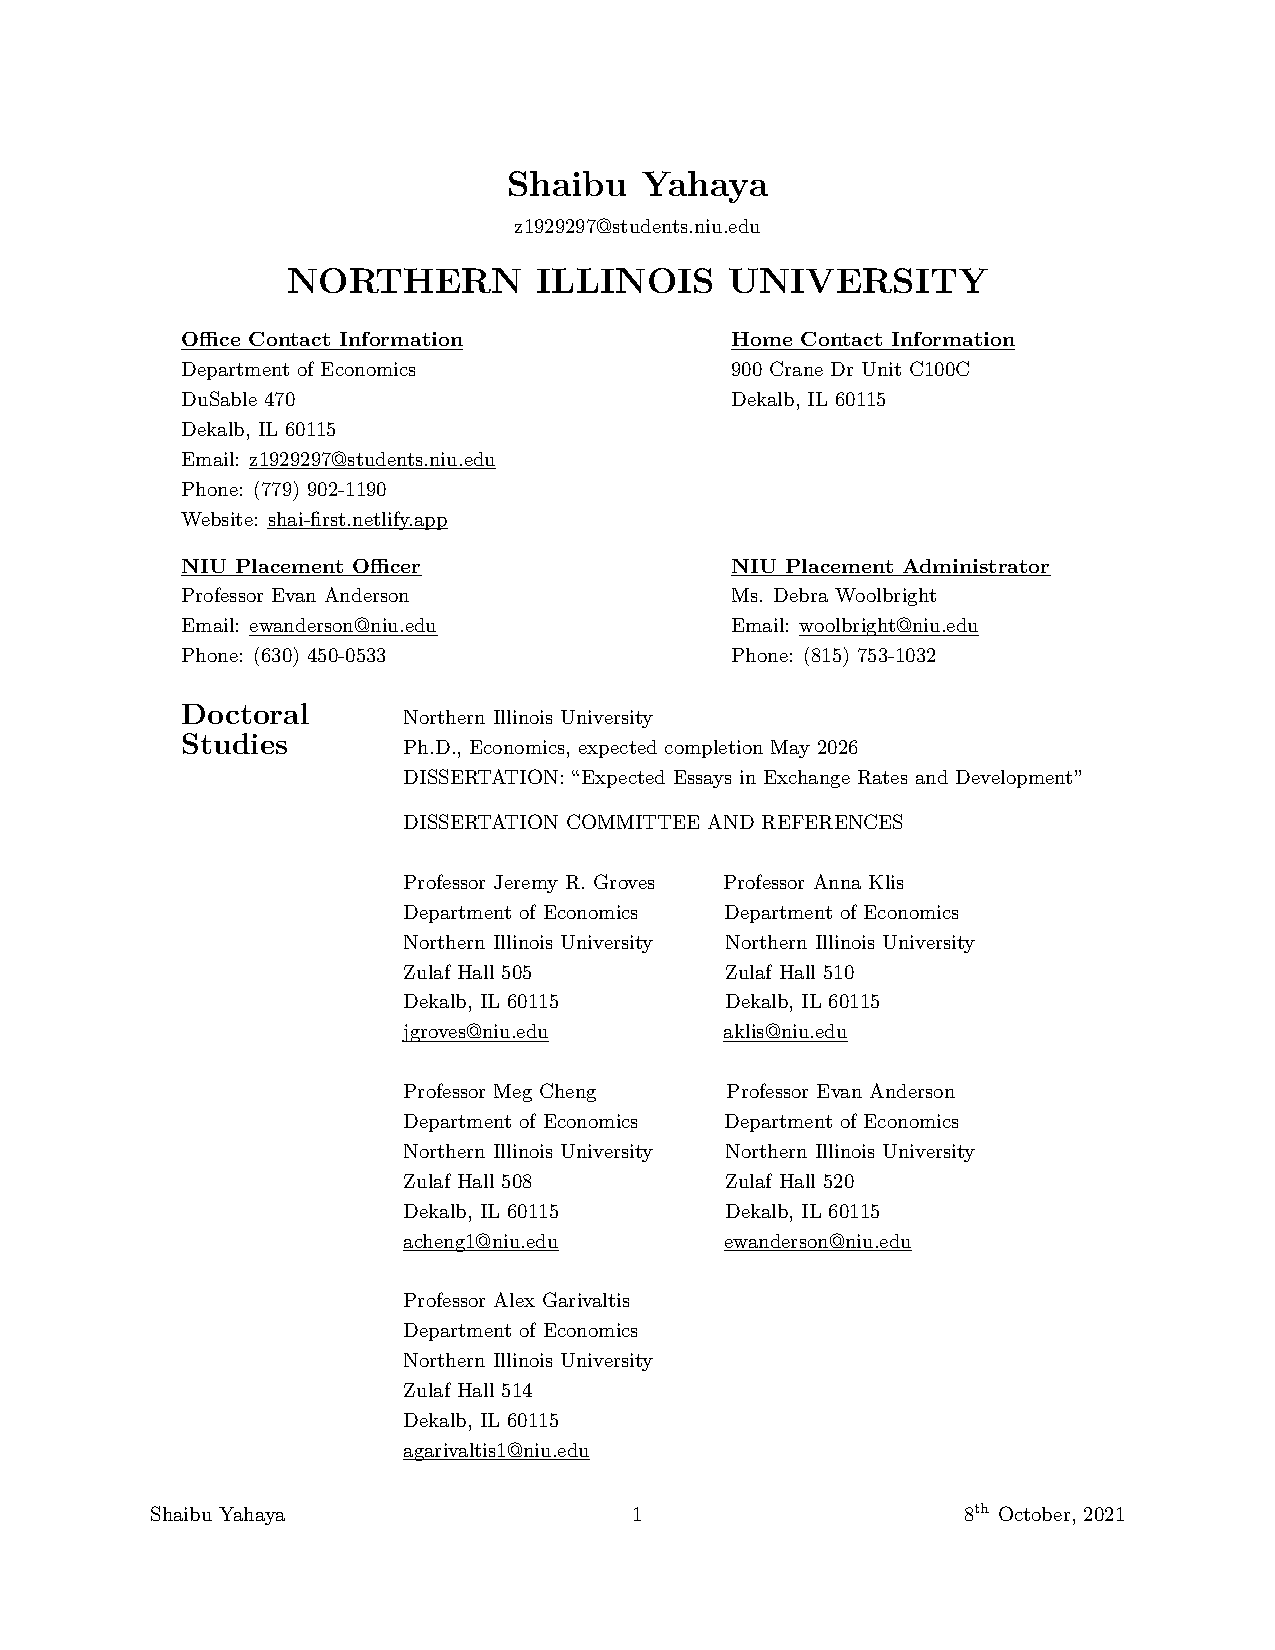
\includegraphics[width=0.25\textwidth]{shai.jpg}
%\end{wrapfigure}
\centering
Thank You
\end{frame}

\end{document}